\documentclass[
11pt, % The default document font size, options: 10pt, 11pt, 12pt
codirector, % Uncomment to add a codirector to the title page
]{charter} 




% El títulos de la memoria, se usa en la carátula y se puede usar el cualquier lugar del documento con el comando \ttitle
\titulo{Control de acceso vehicular} 

% Nombre del posgrado, se usa en la carátula y se puede usar el cualquier lugar del documento con el comando \degreename
\posgrado{Carrera de Especialización en Internet de las cosas} 
%\posgrado{Carrera de Especialización en Internet de las Cosas} 
%\posgrado{Carrera de Especialización en Intelegencia Artificial}
%\posgrado{Maestría en Sistemas Embebidos} 
%\posgrado{Maestría en Internet de las cosas}

% Tu nombre, se puede usar el cualquier lugar del documento con el comando \authorname
\autor{Jose Mauricio Lara Tapia} 

% El nombre del director y co-director, se puede usar el cualquier lugar del documento con el comando \supname y \cosupname y \pertesupname y \pertecosupname
\director{Ariel Lutenberg}
\pertenenciaDirector{FIUBA,CONICET} 
% FIXME:NO IMPLEMENTADO EL CODIRECTOR ni su pertenencia
\codirector{Lionel Gutierrez} % para que aparezca en la portada se debe descomentar la opción codirector en el documentclass
\pertenenciaCoDirector{FIUBA}

% Nombre del cliente, quien va a aprobar los resultados del proyecto, se puede usar con el comando \clientename y \empclientename
\cliente{Jose Mauricio Lara Tapia}
\empresaCliente{Estudiante CEIot}

% Nombre y pertenencia de los jurados, se pueden usar el cualquier lugar del documento con el comando \jurunoname, \jurdosname y \jurtresname y \perteunoname, \pertedosname y \pertetresname.
\juradoUno{Nombre y Apellido (1)}
\pertenenciaJurUno{pertenencia (1)} 
\juradoDos{Nombre y Apellido (2)}
\pertenenciaJurDos{pertenencia (2)}
\juradoTres{Nombre y Apellido (3)}
\pertenenciaJurTres{pertenencia (3)}
 
\fechaINICIO{30 de abril de 2021}		%Fecha de inicio de la cursada de GdP \fechaInicioName
\fechaFINALPlan{18 de junio de 2021} 	%Fecha de final de cursada de GdP
\fechaFINALTrabajo{15 de mayo de 2022}	%Fecha de defensa pública del trabajo final


\begin{document}

\maketitle
\thispagestyle{empty}
\pagebreak


\thispagestyle{empty}
{\setlength{\parskip}{0pt}
\tableofcontents{}
}
\pagebreak


\section{Registros de cambios}
\label{sec:registro}


\begin{table}[ht]
\label{tab:registro}
\centering
\begin{tabularx}{\linewidth}{@{}|c|X|c|@{}}
\hline
\rowcolor[HTML]{C0C0C0} 
Revisión & \multicolumn{1}{c|}{\cellcolor[HTML]{C0C0C0}Detalles de los cambios realizados} & Fecha      \\ \hline
0      & Creación del documento                                 &\fechaInicioName \\ \hline
%1      & Se completa hasta el punto 4 inclusive                 & dd/mm/aaaa \\ \hline
%2      & Se completa hasta el punto 7 inclusive
%		  Se puede agregar algo más \newline
%		  En distintas líneas \newline
%		  Así                                                    & dd/mm/aaaa \\ \hline
%3      & Se completa hasta el punto 11 inclusive                & dd/mm/aaaa \\ \hline
%4      & Se completa el plan	                                 & dd/mm/aaaa \\ \hline
\end{tabularx}
\end{table}

\pagebreak



\section{Acta de constitución del proyecto}
\label{sec:acta}

\begin{flushright}
Buenos Aires, \fechaInicioName
\end{flushright}

\vspace{2cm}

Por medio de la presente se acuerda con el Ing. \authorname\hspace{1px} que su Trabajo Final de la \degreename\hspace{1px} se titulará ``\ttitle'', consistirá esencialmente en \textcolor{black}{en desarrollo de un sistema de software y prototipo preliminar para control de acceso vehicular }, y tendrá un presupuesto preliminar estimado de \textcolor{black}{640} hs de trabajo y \textcolor{black}{7218 USD}, con fecha de inicio \fechaInicioName\hspace{1px} y fecha de presentación pública \fechaFinalName.

Se adjunta a esta acta la planificación inicial.

\vfill

% Esta parte se construye sola con la información que hayan cargado en el preámbulo del documento y no debe modificarla
\begin{table}[ht]
\centering
\begin{tabular}{ccc}
\begin{tabular}[c]{@{}c@{}}Ariel Lutenberg \\ Director posgrado FIUBA\end{tabular} & \hspace{2cm} & \begin{tabular}[c]{@{}c@{}}\clientename \\ \empclientename \end{tabular} \vspace{2.5cm} \\ 
\multicolumn{3}{c}{\begin{tabular}[c]{@{}c@{}} \supname \\ Director del Trabajo Final\end{tabular}} \vspace{2.5cm} \\
%\begin{tabular}[c]{@{}c@{}}\jurunoname \\ Jurado del Trabajo Final\end{tabular}     &  & \begin{tabular}[c]{@{}c@{}}\jurdosname\\ Jurado del Trabajo Final\end{tabular}  \vspace{2.5cm}  \\
%\multicolumn{3}{c}{\begin{tabular}[c]{@{}c@{}} \jurtresname\\ Jurado del Trabajo Final\end{tabular}} \vspace{.5cm}                                                                     
\end{tabular}
\end{table}

\section{Descripción técnica-conceptual del proyecto a realizar}
\label{sec:descripcion}
\begin{consigna}{black} % El bloque "consigna" se usa para poner texto en rojo y dar una pequeña ayuda sobre cómo completar la sección
Cada vez es más común encontrar nuevas organizaciones como centros comerciales, edificios y zonas residenciales. que están sujetos a tener concurrencia vehicular. Esto implica tener una administración que gestione la organización y control de circulación por los diferentes ambientes. 

Hoy en día encontramos diferentes tecnologías para este tipo de tareas que por lo general en nuestro medio son sistemas  importados que no llegan a encajar con los requerimientos actuales como digitalización de información, autonomía en el sistema control de acceso y  monitoreo de actividades de circulación en los ambientes.

De esta manera se genera un proyecto basado en la premisa de digitalización y automatización de las tareas en lo que respecta control de acceso vehicular.
 
El sistema busca dar una mejor eficiencia y comodidades hacia los usuarios,mediante la tecnología RFID UHF. Esta tecnología ha sido desarrollada para aplicaciones de control de acceso pasivo que a comparación de los sistemas actuales  basados en RFID, proveen una solución más sencilla y eficiente además ofrece una mayor versatilidad para una gran gama de soluciones.


La finalidad de este proyecto es desarrollar un sistema que adopte el paradigma de internet de las cosas.

El sistema de control de acceso posera primordialmente un lector UHF RFID, el cual estará comunicado con un microcontrolador. El microcontrolador estará encargado de esperar los datos que constan de la identificación del tag RFID.Cuando se identifique un código de algún tag  se enviará esto a un broker. El broker a su vez retransmite a un nodo (node JS) lo cual  consultará a una base de datos sobre el código leído del tag. Se recibirá una respuesta de la base de datos y el nodo evaluará si el usuario con ese tag tiene acceso. El nodo retransmite el mensaje de acceso o no acceso al broker y el broker a microcontrolador que permitirá o no  el acceso.

En la figura 1. se presenta el esquema de comunicación entre los diferentes componentes del sistema.
%\vspace{25px}

\begin{figure}[htpb]
\centering 
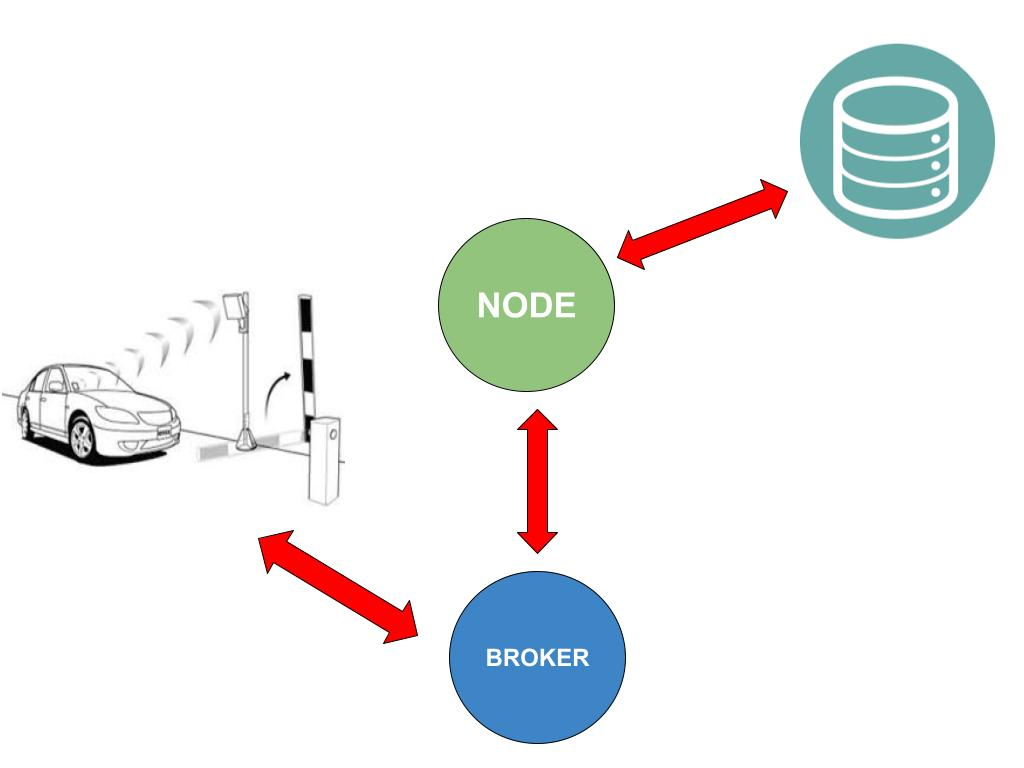
\includegraphics[width=12cm, height=8cm]{./Figuras/ESQ.jpg}
\caption{Esquema de comunicaciona del sistema}
\label{fig:diagBloques}
\end{figure}

\vspace{25px}

En la Figura 2 se presenta el diagrama de bloques con sus diferentes elementos a nivel sistema  
\begin{figure}[htpb]
\centering 
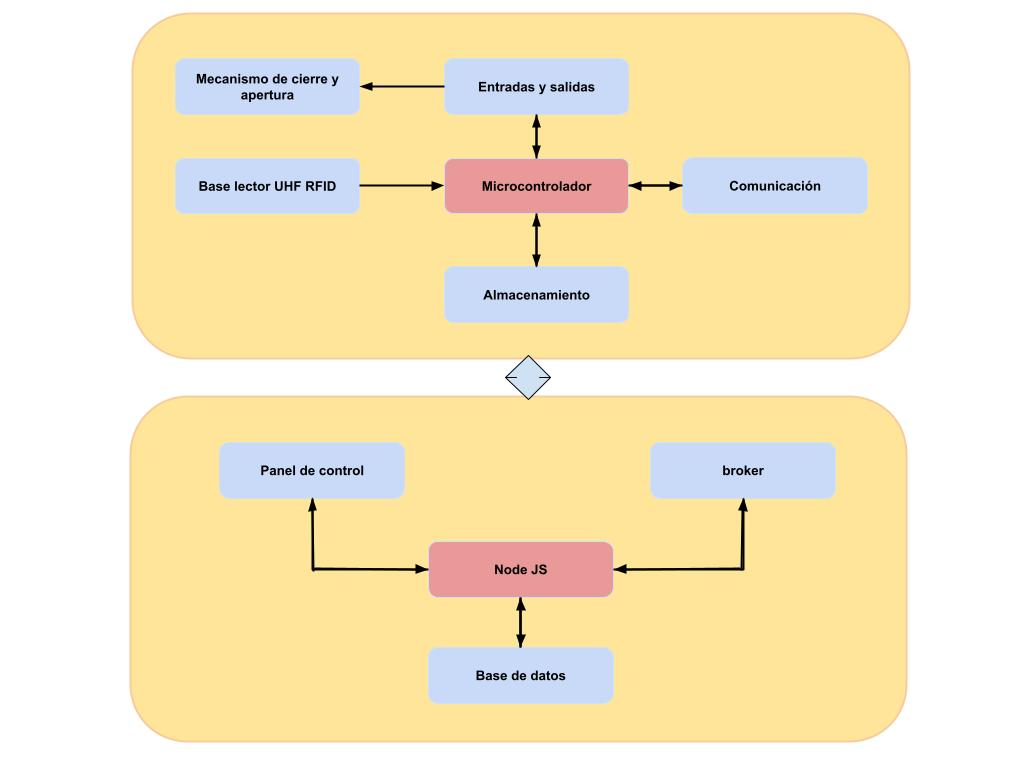
\includegraphics[width=15cm, height=12cm]{./Figuras/DIAGBLOQ.jpg}
\caption{Diagrama en bloques del sistema}
\label{fig:diagBloques}
\end{figure}
\end{consigna}
\section{Identificación y análisis de los interesados}
\label{sec:interesados}
\begin{consigna}{black} 
\begin{table}[ht]
%\caption{Identificación de los interesados}
%\label{tab:interesados}
\begin{tabularx}{\linewidth}{@{}|l|X|X|l|@{}}
\hline
\rowcolor[HTML]{C0C0C0} 
Rol           & Nombre y Apellido & Organización 	& Puesto 	\\ \hline
Cliente       & Jose Mauricio Lara Tapia            &\empclientename	&   Cliente	\\ \hline
Responsable   & \authorname       & FIUBA        	& Alumno 	\\ \hline
Colaboradores & Lionel Gutierrez  & FIUBA           & Codirector       	\\ \hline
Orientador    & \supname	      & \pertesupname 	& Director Trabajo final \\ \hline
Usuario final & Personas adulta   &              	& Clientes   	\\ \hline
\end{tabularx}
\end{table}

\end{consigna}
\section{1. Propósito del proyecto}
\label{sec:proposito}
El proposito de presente proyecto es desarrollar un prototipo de una nueva version de sistema de control de acceso vehicular utilizando tecnolgia UHF RFID y adoptando el paradigma IOT
\begin{consigna}{red}
\end{consigna}
\section{2. Alcance del proyecto}
\label{sec:alcance}
\begin{consigna}{black}
El presente proyecto incluye:
\begin{itemize}
	\item Prototipo del equipo funcionando.
	\item Documentacion del firmware del equipo.
	\item Plataforma con servicios forntend y backend.

\end{itemize}
\end{consigna}
\begin{consigna}{black}
El presente proyecto no incluye:
\begin{itemize}
	\item Desarrollo de hardware o PCB.
	\item Manual de instalacion y uso.
	\item Desarrollo de aplicaciones moviles.
	\item Mecanismo de apertura para vehiculos.
\end{itemize}
\end{consigna}
\section{3. Supuestos del proyecto}
\label{sec:supuestos}
\begin{consigna}{black}
Para el desarrollo del presente proyecto se supone que:
\begin{itemize}
	\item Se dispondrá de los fondos presupuestados para la compra de insumos y materiales.
	\item No ocurrirán eventos fortuitos que limiten la cantidad de horas propuestas para el proyecto.
\end{itemize}
\end{consigna}
\section{4. Requerimientos}
\label{sec:requerimientos}
\begin{consigna}{black}
Los requerimientos para el desarrollo del proyecto son los siguientes:
\begin{enumerate}
	\item Requerimientos de documentación
		\begin{enumerate}
			\item Se debe generar una Memoria Técnica con la documentación de ingeniería detallada.
			\item Se debe generar un documento de casos de prueba.
		\end{enumerate}
	\item Requerimientos funcionales
		\begin{enumerate}
		\item El sistema debe leer el numero de serie de los tags 'UHF RFID'.
		\item El sistema debe contar con un panel de control para monitorizacion de los eventos y control del equipo.
		\item el sistema contara con un registro de los tags autorizados.
		\item El sistema debe generar alertas ante acciones de autorizacion y denegacion de acceso.
		\item El sistema debe detectar si el acceso vehicular se encuentra en estado de apertura o cierre.
		\item El sistema debe tener dos modos de operacion, lectura de tags o password de administrador en caso de eventos imprevistos.
		\item El sistema debe permitir identificar crear y borrar usuarios
del sistema.
		\end{enumerate}
	\item Requerimientos no funcionales:
		\begin{enumerate}
		\item El sistema deberá ser escalable, de forma de poder agregar más funcionalidades a futuro.
		\item  El código del proyecto debe trabajarse bajo un sistema de control de versiones git con repositorio en la nube tipo github o similar.
		    \end{enumerate}
	\item Requerimientos de hardware:
		\begin{enumerate}
		\item Se contara con un modulo lector de tags 'UHF RFID'.
		\item Se contara con alarma sonora.
		\item Se contara con un actudor tipo rele.
		\item Se utilizará una placa de desarrollo embebida comercial para control central del proyecto.
		    \end{enumerate}
		\begin{enumerate}
		\end{enumerate}
\end{enumerate}
\end{consigna}
\section{5. Historias de usuarios (\textit{Product backlog})}
\label{sec:backlog}
Para determinar los storypoints de las historias de usuario se toma en cuenta los siguientes
aspectos:
\begin{consigna}{black}
\begin{enumerate}
	\item Cantidad de trabajo a realizar.
		\begin{enumerate}
			\item Bajo = 3 pts.
			\item Medio = 8 pts.
			\item Alto = 13 pts.
		\end{enumerate}
		\item Complejidad del trabajo a realizar.
		\begin{enumerate}
			\item Bajo = 3 pts.
			\item Medio = 8 pts.
			\item Alto = 13 pts.
		\end{enumerate}
			\item Riesgo o incertidumbre del trabajo a realizar.
		\begin{enumerate}
			\item Bajo = 3 pts.
			\item Medio = 8 pts.
			\item Alto = 13 pts.
		\end{enumerate}
\end{enumerate}
\begin{itemize}
    \item  Roles:
\begin{itemize}
	\item Usuario Central: Es el que gestiona el sistema de control de acceso vehicular .
	\item Usuario vehiculo : Usuario que forma parte de la organizacion.
\end{itemize}
\item  Historias de usuario:
\begin{itemize}
	\item Como usuario Central quiero poder detectar a los usuarios con acceso en base al tag 'UHF RFID'. (8pts+8pts+3pts=19pts)
	\item Como usuario central quiero verificar la informacion del usuario con el panel de control en tiepo real. (8pts+8pts+8pts=24) 
	\item Como usuario central quiero poder dar de alta nuevos usuarios de la organizacion.
	 (13pts+8pts+8pts=29)
	\item como usuario central quiero obtener notificaciones de las acciones de apertura y cierre de la zona de acceso en tiempo real. (8pts+8pts+8pts=24pts)
	\item Como usaurio central quiero obtener alertas cuando la zona de acceso este mucho tiempo en estado de apertura o cierre. (8pts+8pts+8pts=24pts)
	\item Como usuario central quiero tener control de apertura por password ante eventos inesperados. (13pts+13pts+8pts=34pts)
	\item Como usuario cetral debo poder solicitar, modificar y borrar  la info de los registros. (8pts+8ts+8pts=24pts)
	\item Como de vehiculo debo poder tener acceso a los ambientes con mi tag 'UHF RFID'. 
	(8pts+3pts+3pts=14pts)
\end{itemize}
\end{itemize}
\end{consigna}
\section{6. Entregables principales del proyecto}
\label{sec:entregables}
\begin{consigna}{black}
Los entregables principales del proyecto son:
\begin{itemize}
	\item Diagrama esquematico del harware del equipo.'
	\item Código fuente del firmware para control del equipo.
	\item Prototipo del equipo funcionando.
	\item Informe final del proyecto.
\end{itemize}
\end{consigna}
\section{7. Desglose del trabajo en tareas}
\label{sec:wbs}
A continuación se puede evidenciar la planificación de horas correspondientes al proyecto:
\begin{consigna}{black}
\begin{enumerate}
\item Planificacion del proyecto (70 hs)
	\begin{enumerate}
	\item Realizar plan de proyecto (20 hs)
	\item Especificación de requisitos del proyecto (20 hs)
	\item Viabilidad económica y financiera del proyecto (30 hs)
	\end{enumerate}
\item  Investigacion preliminar (60 hs)
	\begin{enumerate}
	\item Buscar info. sobre sistemas de control de accesos por parametros RFID. (10 hs)
	\item Buscar info. sobre los modulos de 'UHF RFID' . (10 hs)
	\item Buscar info sobre plataformas ara desarrollo de dashboards  (10 hs)
	\item Buscar ifo. sobre alternativas de brockers MQTT disponibles  (10 hs).
	\item Buscar info de tecnologia para desarrollo de aplicaciones backend y  (10 hs). 
	\item Buscar info. sobre tecnologias para modelado de bases de datos. (10 hs)
	\end{enumerate}
\item Gestion de compras de modulos comerciales para el proyecto. (10 hs)
	\begin{enumerate}
	\item Adquisicion de componentes. (10 hs)
	\end{enumerate}
\item Diseno e implementacion de aplicacion web. ( 230 hs)
	\begin{enumerate}
	\item configuracion del brocker. (40 hs)
	\item Configuracion de plataforma para desarollo de dashboard. (50 hs)
	\item configuracion de plataforma para desarrollo de aplicacion backend. (40 hs)
	\item Análisis y Diseño del modelo de datos/Base de Datos. ( 50 hs)
	\item Diseno del servicio de ingreso, modificacion y borrado de datos. ( 50 hs)
	\end{enumerate}
\item Desarrollo de firmware para los modulos del sistema . (140 hs)
	\begin{enumerate}
	\item Diseno de arquitectura del firmware. ( 40 hs)
	\item Programacion de funciones para obtencion de lectura del modulo 'UHD RFID'. (15)
	\item Programacion de funciones para modulo actuador y alarmas sonora. ( 15 hs)
	\item Programacion de funciones para la comunicacion con aplicacion web (40 hs)
	\item Integracion de firmware completo. (30hs)
	\end{enumerate}
\item Procesos finales del proyecto. (140 hs)
	\begin{enumerate}
	\item Pruebas de funcionalidad y correccion de errores. (50 hs)
	\item Elaboracion de informe de avance. ( 25 hs)
	\item Elaboracion de memoria de proyecto. (40)
	\item Preparacion de la presentacion del proyecto fina. (25)
	\end{enumerate}
\end{enumerate}
\end{consigna}

\section{8. Diagrama de Activity On Node}
\label{sec:AoN}

\begin{consigna}{red}


%La figura \ref{fig:AoN} fue elaborada con el paquete latex tikz y pueden consultar la siguiente referencia \textit{online}:

%\url{https://www.overleaf.com/learn/latex/LaTeX_Graphics_using_TikZ:_A_Tutorial_for_Beginners_(Part_3)\%E2\%80\%94Creating_Flowcharts}

\end{consigna}

\begin{figure}[htpb]
\centering 
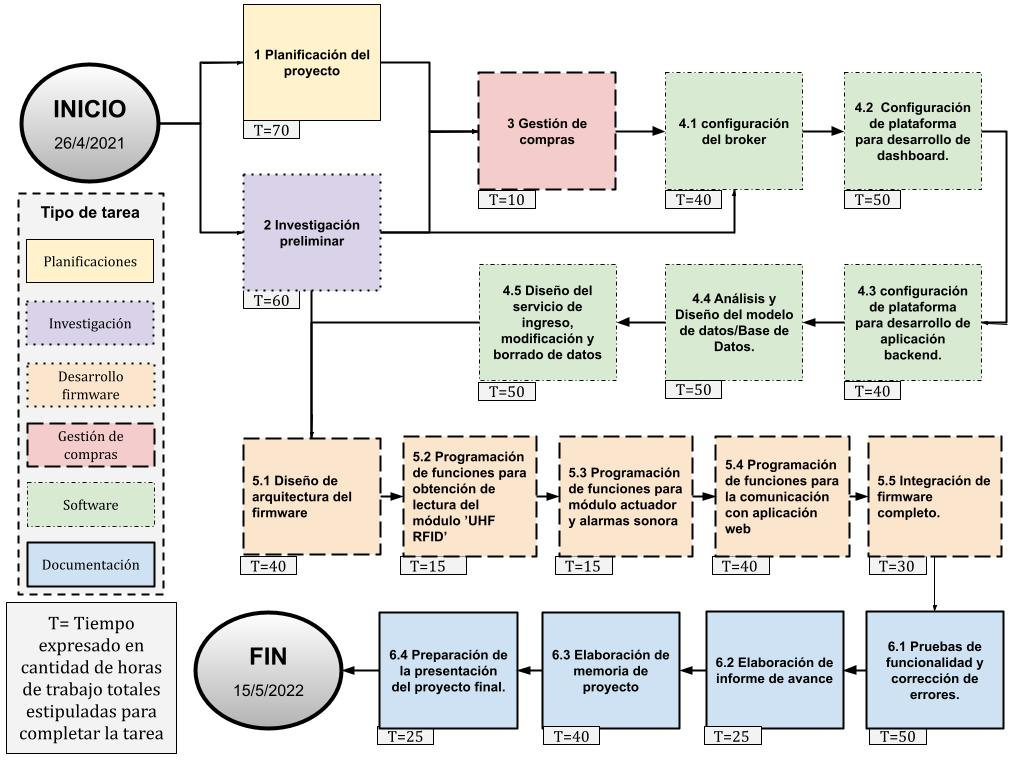
\includegraphics[width=16cm, height=18cm]{./Figuras/DAoN.jpg}
\caption{Diagrama en \textit{Activity on Node}}
\label{fig:AoN}
\end{figure}




\section{9. Diagrama de Gantt}
\label{sec:gantt}
En la Figura 4, se muestra las actividades y la cantidad de dı́as para el diagrama de Gantt
propuesto en base al desglose del trabajo en tareas.
\begin{consigna}{black}
\begin{figure}[htpb]
\centering 
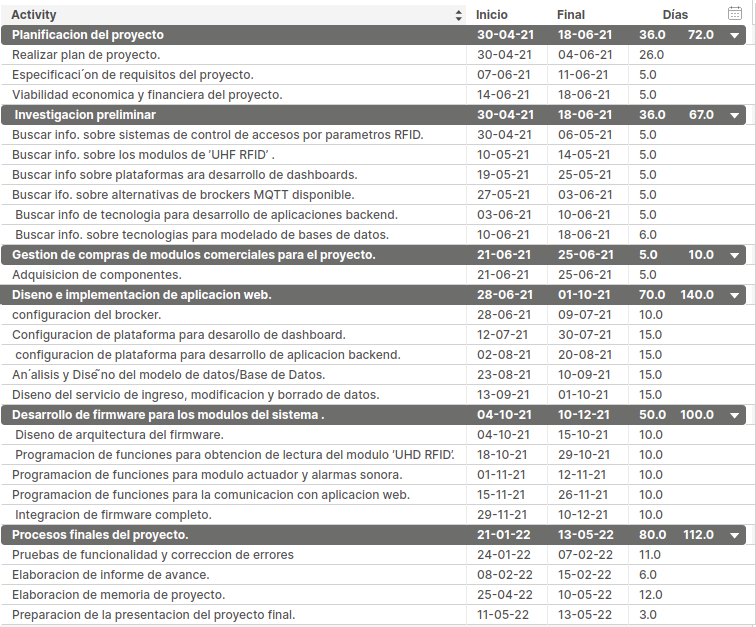
\includegraphics[width=16cm, height=18cm]{./Figuras/Listadiagramadegant.png}
\caption{Actividades del diagrama de gantt}
\label{fig:AoN}
\end{figure}


En la Figura 5, se muestra el diagrama de Gantt propuesto en base al desglose del trabajo en
tareas.

\begin{figure}[htpb]
\centering 
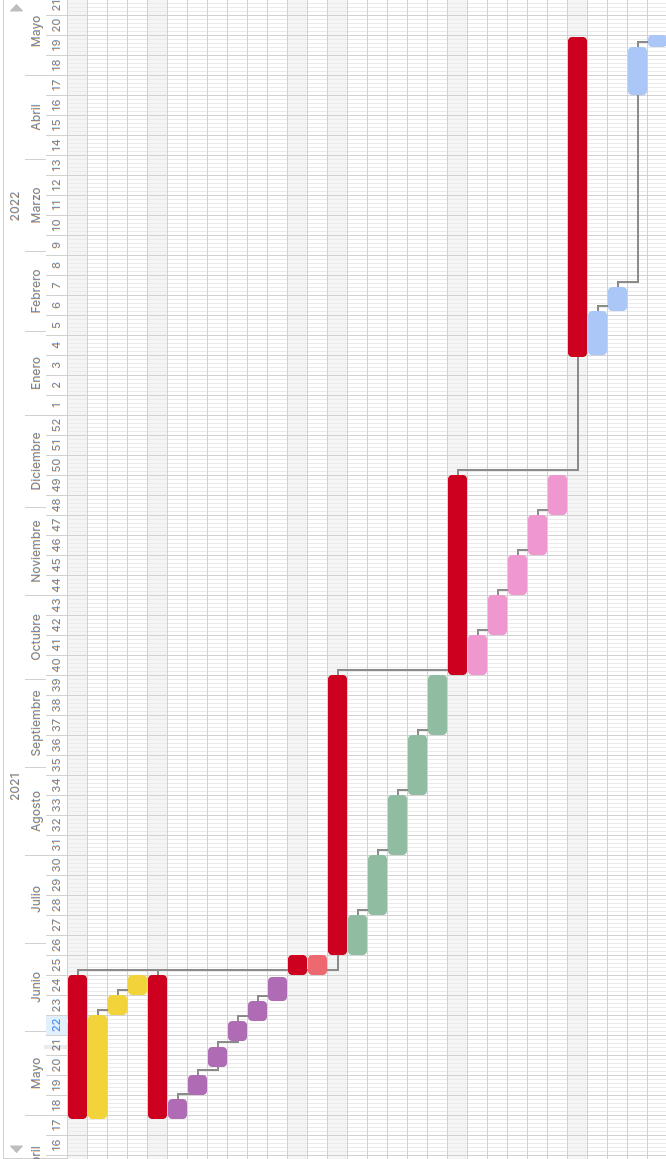
\includegraphics[width=16cm, height=18cm]{./Figuras/digrama de gantt.png}
\caption{Actividades del diagrama de gantt}
\label{fig:AoN}
\end{figure}

\end{consigna}


\section{10. Presupuesto detallado del proyecto}
\label{sec:presupuesto}

\begin{consigna}{black}
En la siguiente tabla se puede observar el presupuesto detallado del proyecto expresado en
dólares.
\end{consigna}

\begin{table}[htpb]
\centering
\begin{tabularx}{\linewidth}{@{}|X|c|r|r|@{}}
\hline
\rowcolor[HTML]{C0C0C0} 
\multicolumn{4}{|c|}{\cellcolor[HTML]{C0C0C0}COSTOS DIRECTOS} \\ \hline
\rowcolor[HTML]{C0C0C0} 
Descripción &
  \multicolumn{1}{c|}{\cellcolor[HTML]{C0C0C0}Cantidad} &
  \multicolumn{1}{c|}{\cellcolor[HTML]{C0C0C0}Valor unitario USD} &
  \multicolumn{1}{c|}{\cellcolor[HTML]{C0C0C0}Valor total USD} \\ \hline
  Mano de obra directa 
 &
  \multicolumn{1}{c|}{640 hs} &
  \multicolumn{1}{c|}{10} &
  \multicolumn{1}{c|}{6400} \\ \hline
  Placa de desarrollo embebida 
 &
  \multicolumn{1}{c|}{2 u} &
  \multicolumn{1}{c|}{12} &
  \multicolumn{1}{c|}{24} \\ \hline
  Componentes electronicos
 &
 \multicolumn{1}{c|}{2 u} &
  \multicolumn{1}{c|}{N/A} &
  \multicolumn{1}{c|}{50} \\ \hline
  Herramientas varias 
&
 \multicolumn{1}{c|}{2 u} &
  \multicolumn{1}{c|}{N/A} &
  \multicolumn{1}{c|}{50} \\ \hline

\multicolumn{3}{|c|}{SUBTOTAL} &
  \multicolumn{1}{c|}{6524} \\ \hline
\rowcolor[HTML]{C0C0C0} 
\multicolumn{4}{|c|}{\cellcolor[HTML]{C0C0C0}COSTOS INDIRECTOS} \\ \hline
\rowcolor[HTML]{C0C0C0} 
Descripción &
  \multicolumn{1}{c|}{\cellcolor[HTML]{C0C0C0}Cantidad} &
  \multicolumn{1}{c|}{\cellcolor[HTML]{C0C0C0}Valor unitario USD} &
  \multicolumn{1}{c|}{\cellcolor[HTML]{C0C0C0}Valor total USD} \\\hline
  Electricidad&
  \multicolumn{1}{c|}{640 hs} &
  \multicolumn{1}{c|}{0.10} &
  \multicolumn{1}{c|}{64} \\ \hline
Telefonia &
     \multicolumn{1}{c|}{60 hs} &
  \multicolumn{1}{c|}{0.50} &
  \multicolumn{1}{c|}{30} \\ \hline

Mano de obra indirecta &
     \multicolumn{1}{c|}{N/A} &
  \multicolumn{1}{c|}{N/A} &
  \multicolumn{1}{c|}{600} \\ \hline

 
\multicolumn{3}{|c|}{SUBTOTAL} &
  \multicolumn{1}{c|}{694} \\ \hline
\rowcolor[HTML]{C0C0C0}
\multicolumn{3}{|c|}{TOTAL} &7218
   \\ \hline
\end{tabularx}%
\end{table}


\section{11. Gestión de riesgos}
\label{sec:riesgos}

\begin{consigna}{black}
a) Identificación de los riesgos y estimación de sus consecuencias:
 
Riesgo 1: Fallas de los componentes que conforma el sistema.
\begin{itemize}
	\item Severidad (S) : 6. Este riego puede retrasar las tareas que se va realizar en el proyecto hasta encontrar la solución.
	\item Probabilidad de ocurrencia (O): 4 Las plataformas de hardware pueden llegar a fallar por accidentes por fatiga o accidentes.

\end{itemize}   

Riesgo 2: La planificación de las horas de trabajo insuficientes para alcanzar la fecha de entrega.

\begin{itemize}
	\item Severidad (S):  9. Esta severidad  implicaría un retraso en la entrega del proyecto.
	\item Ocurrencia (O):3. Se ha dedicado mucha atención para definir la duración de tareas.
\end{itemize}

Riesgo 3: No cumplir con el alcance del proyecto.
\begin{itemize}
	\item Severidad (S): 9. Esta severidad se debería  por la falta de tiempo o dedicación al proyecto.
	\item Ocurrencia (O):4. Cargas de trabajo de la fuente laboral  por parte del encargado del proyecto.
\end{itemize}

Riesgo 4: Problemas personales que se presenten de manera imprevista que impidan continuar con el proyecto.
\begin{itemize}
	\item Severidad (S): 9. Esta severidad retrasa todo el proyecto porque afecta las prioridades del responsable dejando de lado las actividades establecidas del proyecto hasta su solución.
	\item Ocurrencia (O): 3. Cargas de trabajo de la fuente laboral  por parte del encargado del proyecto.
\end{itemize}

Riesgo 5: Pérdida de trabajo ya realizado (software, firmware) causada por rotura o pérdida del almacenamiento local que lo contiene.
\begin{itemize}
	\item Severidad (S):  9. Se perdería todo el trabajo y avance realizado.
	\item Ocurrencia (O):4. Es un problema bastante común pero la frecuencia en que ocurre es baja.
\end{itemize}

b) Tabla de gestión de riesgos:      (El RPN se calcula como RPN=SxO)

\begin{table}[htpb]
\centering
\begin{tabularx}{\linewidth}{@{}|X|c|c|c|c|c|c|@{}}
\hline
\rowcolor[HTML]{C0C0C0} 
Riesgo & S & O & RPN & S* & O* & RPN* \\ \hline
    Fallas de los componentes que conforma el sistema   & 6  & 4  &  24  & 3   & 4   &12      \\ \hline
    La planificación de las horas de trabajo insuficientes para alcanzar la fecha de entrega.   &  9 & 3  &  27   &  6  & 3   &  18    \\ \hline
    No cumplir con el alcance del proyecto.  &  9 & 3  &  27   &  6  &   3 &   18   \\ \hline
    Problemas personales que se presenten de manera imprevista que impidan continuar con el proyecto.  &  9 &  2 &  18   &  -  & -   &   -   \\ \hline
    Pérdida de trabajo ya realizado (software, firmware) causada por rotura o pérdida del almacenamiento local que lo contiene.   &  9 & 3  &   27  &   6 &   3 &    18  \\ \hline
\end{tabularx}%
\end{table}

Criterio adoptado: 
El RPN tolerable es de 18. Se tomarán medidas de mitigación para los RPN mayores a 18.

Nota: los valores marcados con (*) en la tabla corresponden luego de haber aplicado la mitigación.

c) Plan de mitigación de los riesgos que originalmente excedían el RPN máximo establecido:
 
Mitigacion de riesgo 1: Se realizara el remplazo de componentes fallidos
\begin{itemize}
	\item Severidad (S):  2. Baja la severidad porque se mantendra en contacto con provedores para rapidas soluciones.
	\item Probabilidad de ocurrencia (O):4. No se modifica.
\end{itemize}

Mitigacion de riesgo 2: Se trabajarán más horas en el proyecto.
\begin{itemize}
	\item Severidad (S):  6.  Si bien baja un poco la severidad podría incrementar el estrés del responsable causando que el riesgo 4 aumente de probabilidad.
	\item Probabilidad de ocurrencia (O):3. No se modifica.
\end{itemize}
Mitigacion de riesgo 3: Se trabajarán más horas en el proyecto.
\begin{itemize}
	\item Severidad (S):  6.  Si bien baja un poco la severidad podría incrementar el estrés del responsable causando que el riesgo 4 aumente de probabilidad.
	\item Probabilidad de ocurrencia (O):3. No se modifica.
\end{itemize}
Mitigacion de riesgo 5:Se trabajarán los archivos del proyecto directamente “en la nube” (GitHub,Google Drive, etc). Se harán backups semanales en almacenamiento local.

\begin{itemize}
	\item Severidad (S):  6. Los archivos perdidos en almacenamiento local serán fácilmente recuperables.
	\item Probabilidad de ocurrencia (O):3. No se modifica.
\end{itemize}
\end{consigna}
\section{12. Gestión de la calidad}
\label{sec:calidad}

\begin{consigna}{black}
Para cada uno de los requerimientos del proyecto indique:
\begin{itemize} 
\item Req \#1.1: Se debe generar una memoria técnica con documentación del proyecto
\begin{itemize}
	\item Verificación: Durante las diferentes etapas del proyecto se establece procesos de desarrollo que contemple la generación de documentación.

	\item Validación: Lectura y revisión de la  memoria técnica por parte del director y los jurados.
\end{itemize}
\item Req \#1.2: Se debe generar un documento con el plan de pruebas del proyecto. 
\begin{itemize}
	\item Verificación: Durante la primera etapa del proyecto se realizará una planificación específica mediante una puesta en común con todos los interesados.
	\item Validación: Lectura y revisión del documento de casos de prueba por parte del cliente y el equipo de trabajo.
\end{itemize}
\item Req \#2.1: El sistema debe leer el numero de serie de los tags ’UHF RFID’
\begin{itemize}
	\item Verificacion: Se realizará un archivo de descripción de funciones en un formato independiente del lenguaje de programación.
	\item Validación: se hará una inspección con el codirector y el director.
\end{itemize}
\item Req \#2.2: El sistema debe contar con un panel de control para monitorizacion de los eventos y control del equipo.
\begin{itemize}
	\item Verificacion: Se realizará un archivo de descripción de funciones en un formato independiente de la plataforma de desarrollo.
	\item Validación: Se hará una inspección con el codirector y el director.
\end{itemize}
\item Req \#2.3: El sistema contara con un registro de los tags autorizados.
\begin{itemize}
	\item Verificacion: Se realizará un archivo de descripción de funciones en un formato independiente de la plataforma de desarrollo.
	\item Validación: Se hará una inspección con el codirector y el director.
\end{itemize}
\item Req \#2.4: El sistema debe generar alertas ante acciones de autorizacion y denegacion de acceso.
\begin{itemize}
	\item Verificacion: Se realizará un archivo de descripción de funciones en un formato independiente de la plataforma de desarrollo.
	\item Validación: Se hará una inspección con el codirector y el director.
\end{itemize}
\item Req \#2.5:  El sistema debe detectar si el acceso vehicular se encuentra en estado de apertura ocierre.
\begin{itemize}
	\item Verificacion: Se realizará un archivo de descripción de funciones en un formato independiente de la plataforma de desarrollo.
	\item Validación: Se hará una inspección con el codirector y el director.
\end{itemize}
\item Req \#2.6:  El  sistema  debe  tener  dos  modos  de  operacion,  lectura  de  tags  o  password  deadministrador en caso de eventos imprevistos.
\begin{itemize}
	\item Verificacion: Se realizará un archivo de descripción de funciones en un formato independiente de la plataforma de desarrollo.
	\item Validación: Se hará una inspección con el codirector y el director.
\end{itemize}
\item Req \#2.7: El sistema debe permitir identificar crear y borrar usuarios del sistema.
\begin{itemize}
	\item Verificacion: Se realizará un archivo de descripción de funciones en un formato independiente de la plataforma de desarrollo.
	\item Validación: Se hará una inspección con el codirector y el director.
\end{itemize}
\item Req \#3.1: El  sistema  deber ́a  ser  escalable,  de  forma  de  poder  agregar  m ́as  funcionalidades a futuro
\begin{itemize}
	\item Verificacion: Se realizarán pruebas de carga (volumen) sobre el sistema, simulando varios sensores simultáneos para ver cómo se comporta el mismo.
	\item Validacion: N/A (requerimiento interno).
\end{itemize}
\item Req \#3.2:  El ćodigo del proyecto debe trabajarse bajo un sistema de control de versiones gitcon repositorio en la nube tipo github o similar.
\begin{itemize}
	\item Verififcaion: Se creara un repositorio del proyecto.
	\item Validacion: Se hará una inspección con el codirector y el director.
\end{itemize}
\item Req \#4.1:  Se contara con un modulo lector de tags ’UHF RFID’.
\begin{itemize}
	\item Validacion: Se comprobará mediante la respectiva hoja de datos del módulo seleccionado previamente.
	\item Verificacion:Se realiza la comprobación del funcionamiento del módulo y su eficiencia.
\end{itemize}
\item Req \#4.2:  Se contara con alarma sonora.
\begin{itemize}
	\item Validacion: Se comprobará mediante la respectiva hoja de datos del módulo seleccionado previamente.
	\item Verificacion:Se realiza la comprobación del funcionamiento del módulo y su eficiencia.
\end{itemize}
\item Req \#4.3:   Se contara con un actudor tipo rele.
\begin{itemize}
	\item Validacion: Se comprobará mediante la respectiva hoja de datos del módulo seleccionado previamente.
	\item Verificacion:Se realiza la comprobación del funcionamiento del módulo y su eficiencia.
\end{itemize}
\item Req \#4.4:  Se  utilizar ́a  una  placa  de  desarrollo  embebida  comercial  para  control  central  del proyecto.
\begin{itemize}
	\item Validacion: Se comprobará mediante la respectiva hoja de datos del módulo seleccionado previamente.
	\item Verificacion:Se realiza la comprobación del funcionamiento del módulo y su eficiencia.
\end{itemize}
\end{itemize}
\end{consigna}

\section{13. Procesos de cierre}    
\label{sec:cierre}

\begin{consigna}{black}
Para el cierre del proyecto se contemplarán las siguientes actividades:

\begin{itemize}
	\item Pautas de trabajo que se seguirán para analizar si se respetó el Plan de Proyecto original:
	\begin{itemize}
	    \item Se evaluarán los requerimientos y objetivos planteados de acuerdo al plan de trabajo.
	    \item Se verificará los tiempos de entrega y ejecución.
	\end{itemize}
	\item Identificación de las técnicas y procedimientos útiles e inútiles que se emplearon, y los problemas que surgieron y cómo se solucionaron:
	\begin{itemize}
	    \item Se identificará el uso de herramientas nuevas en caso de ser requeridas.
	\end{itemize}
	\item Indicar quién organizará el acto de agradecimiento a todos los interesados, y en especial al equipo de trabajo y colaboradores:
	  \begin{itemize}
	    \item Se procederá a agradecer a todas las personas que participaron en el proyecto luego
de la defensa pública.
	\end{itemize}
\end{itemize}

\end{consigna}


\end{document}
